\section{Проектирование веб-приложения для организации и анализа рабочего и личного времени}

Веб-приложение — клиент-серверное приложение, в котором клиентом выступает браузер, а сервером — веб-сервер. Логика веб-приложения распределена между сервером и клиентом, хранение данных осуществляется, преимущественно, на сервере, обмен информацией происходит по сети. Одним из преимуществ такого подхода является тот факт, что клиенты не зависят от конкретной операционной системы пользователя, поэтому веб-приложения являются кроссплатформенными сервисами

Веб-приложение состоит из клиентской и серверной частей, тем самым реализуя технологию «клиент-сервер». Клиентская часть реализует пользовательский интерфейс, формирует запросы к серверу и обрабатывает ответы от него. Серверная часть получает запрос от клиента, выполняет вычисления, после этого формирует веб-страницу и отправляет её клиенту по сети с использованием протокола HTTP.

На этапе проектирования прежде всего формируются модели данных, основываясь на анализе стратегий использования, процессах, которые будут протекать в приложении, а также выделении сущностей системы и связей между ними. Конечными продуктами проектирования можно считать логическую схему базы данных разрабатываемого приложения и набор спецификаций модулей системы.

Перед разработкой любой системы к ней предъявляется ряд требовний, таких как функционал, который должна предоставлять система, сроки разработки, покрытие системы автоматизированными тестами и возможность расширения системы. Следовательно проектирование можно сформулировать как поиск оптимального решения для удовлетворения всех требований представленных данной системе.

Одним из инструментов проектирования программного обеспечения является унифицированный язык моделирования UML. UML — язык графического описания для объектного моделирования в области разработки программного обеспечения, системного проектирования и отображения организационных структур.

\subsection{Диаграмма вариантов использования}
Диаграмма вариантов использования состоит из актеров, для которых система производит действие, описывающее то, что актер хочет получить в результате [15]. РЫБАТЕКСТ РЫБАТЕКСТ РЫБАТЕКСТ РЫБАТЕКСТ РЫБАТЕКСТ РЫБАТЕКСТ РЫБАТЕКСТ РЫБАТЕКСТ РЫБАТЕКСТ РЫБАТЕКСТ РЫБАТЕКСТ РЫБАТЕКСТ РЫБАТЕКСТ РЫБАТЕКСТ РЫБАТЕКСТ РЫБАТЕКСТ РЫБАТЕКСТ РЫБАТЕКСТ 

\begin{figure}[th]
\centering
  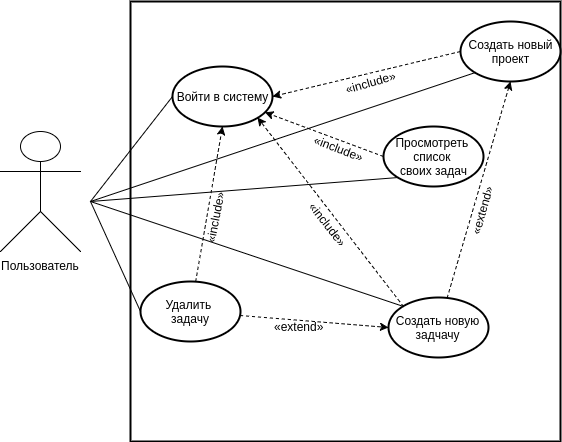
\includegraphics[scale=0.5]{images/diagrams/use-case/1.png}  
  \caption{ Диаграмма сущность-связь для системы организации времени }
  \label{fig:domain:todist}
\end{figure}

\begin{figure}[th]
  \centering
  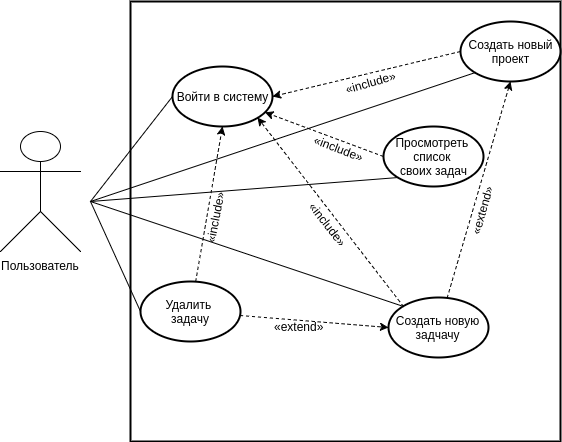
\includegraphics[scale=0.5]{images/diagrams/use-case/1.png}  
  \caption{ Диаграмма сущность-связь для системы организации времени }
  \label{fig:domain:todist}
\end{figure}

\begin{figure}[th]
\centering
  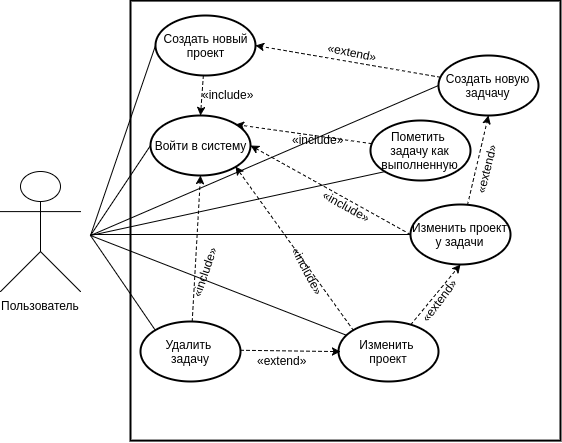
\includegraphics[scale=0.5]{images/diagrams/use-case/3.png} 
  \caption{ Диаграмма вариантов использования проектируемого приложения (продолжение) }
  \label{fig:domain:todist}
\end{figure}

Ниже приведены примеры использования системы пользователем:

1 Создать новую задачу. Перед тем как работать с системой пользователю необходимо авторизоватся в ней. Если пользователь уже был зарегестрирован в системе, он должен выполнить вход, введя свои учетные данные на странице авторизации. Если же пользователь не был зарегистрирован – ему необходимо выполнить регистрацию, а затем авторизоваться, используя указанные им при регистрации данные.

После авторизации в системе пользователь попадает на главную страницу приложения, где он может создать новую задачу. Для того чтобы создать новую задачу пользователь может указать проект для этой задачи. Также он указывает назваие задачи, и ее описание. Для того чтобы следовать метологиям оргнизаации времени "пирамида Франклина" и "матрица Эйзенхауэра" пользователь может указать дополнительные атрибуты - "статус" задчи по "Эйзенхауэру" и "тип" задачи соответственно по "Франклину". По нажатии пользователем кнопки "Создать", данная задача будет определена в соответствующий проект (если он указан), а также автоматически будет сгенерировано время создания задачи.

2 Создать новый проект. Проект представляет из себя группу задач, и используется для категоризации. Для того чтобы создать проект пользователь доллжен нажать на кнопку добавления проекта "+", и ввести название проекта. После добавления проекта пользователь может ассоциировать задачи с данными проектами. 

3 Пометить задачу как "выполненная". Если у пользователя есть активные задачи, он может помить любую из них как "выполненную", отметив это в соответствующем поле в списке задач.